\documentclass[10pt,a4paper]{article}
\usepackage[margin=1in]{geometry}
\usepackage[utf8x]{inputenc}
\usepackage{ucs}
\usepackage[spanish]{babel}
\usepackage{amsmath}
\usepackage{amsfonts}
\usepackage{amssymb}

\usepackage{float}
\usepackage[font=small,labelfont=bf]{caption}
\usepackage{wrapfig}

\usepackage{graphicx}

\usepackage{multicol}

\author{Cristian Escudero}
\title{Resumen SO - II}
\begin{document}
\maketitle
\section{Administración de Memoria}
La \textbf{tarea principal} de cualquier sistema de gestión de memoria es traer los programas a la memoria principal para su ejecución en el procesador. Las técnicas siguientes usan \textbf{paginación pura}, sin \textit{memoria virtual}.

\begin{multicols}{2} 
\textbf{Sin intercambio:}
\begin{itemize}
\item Monoproceso.
\item Multiproceso.
\subitem + Particiones Fijas.
\subitem + Particiones Variables.
\end{itemize}
\columnbreak
\textbf{Con intercambio:}
\begin{itemize}
\item Paginación.
\item Segmentación.
\subitem $ $
\subitem $ $
\end{itemize}
\end{multicols}
 
\paragraph{Sistema monoproceso.} La memoria solo está ocupada por el SO, distribuído entre RAM, ROM, y un único programa. Si la solicitud de memoria es superior a la capacidad disponible, el programa no se ejecuta, informando al sistema de la condición.

\paragraph{Sistema multiproceso.} El SO subdivide la memoria dinámicamente para hacer sitio a varios procesos. Esto se conoce como \textbf{gestión de memoria}.
 
\subparagraph{+ Particiones Fijas.} La memoria es subdividida en áreas de capacidad fijas -de ahí el nombre-. Estas no se modifican durante toda la ejecución del sistema. La gestión consistirá entonces en asignar las particiones según la solicitud de los procesos y conocer que particiones están libres y cuales vacías.

\underline{Dificultad:} Según el método de administración de memoria, será utilizar una \textbf{única cola} de procesos peticionales o \textbf{múltiples colas} asegurando una a cada partición.

\subparagraph{+ Particiones Variables.} El SO arranca con una \textbf{única partición} que ocupa \underline{toda} la capacidad disponible. A medida que los procesos soliciten espacio de memoria, se irán creando las particiones que correspondan, de manera de satisfacer los pedidos recibidos. Cuando no haya más espacio disponible, no podrán hacerse nuevas asignaciones ni ejecutarse nuevos procesos.

\subsection{Reubicación, Protección e Intercambio}

\paragraph{Reubicación.} Pretende mantener indetectable todos los saltos de programa sin importar que ubicación en la memoria se asigne al mismo. Esto se logra considerando todas las instrucciones de salto relativo a la posición que se asigna en la memoria al proceso.

Normalmente la memoria disponible está compartida por varios procesos, por eso se busca poder cargar y descargar procesos activos en la memoria principal. Cuando un programa sea descargado al disco, al volverse a cargar, deberá situarse en la misma posición de memoria que estaba antes.

\paragraph{Protección.} Se refiere a la propiedad que debiera tener un SO para no permitir que un \textbf{proceso sobreescriba un área de memoria} que le correspondiera a otro proceso al mismo SO. Esto podría darse por el solapamiento producido por el crecimiento de interrupciones MOV hacia la memoria. En los sistemas actuales la protección la provee el mismo microprocesador, en lo denominado \textbf{modo protegido}.

\paragraph{Intercambio.} Consiste en llevar o trasladar a una memoria auxiliar procesos o parte de ellos que se encuentran en la memoria principal para poder ejecutar otros (cuando no exista memoria disponible).

Según el SO, el intercambio se realiza sobre un área del disco conformado por un archivo o una partición: \textbf{Pagefile.sys} (\textit{Windows}), \textbf{SWAP} (\textit{Linux}).

\subsection{Técnicas Básicas de Administración de Memoria}

\paragraph{Mapa de Bits.} Se divide a la memoria en un conjunto de \textit{particiones fijas} y se crea un \textbf{mapa de bits}, con tantos \textit{bits} como particiones que se hayan definido: un \textbf{1} indicará a la partición como \textbf{ocupada}, y un \textbf{0} como \textbf{disponible}.

Al momento de solicitar un espeacio en la memoria, el SO deberá revisar el \textit{mapa de bits} para determinar la asignación y si esta es posible. Existen cuatro algoritmos para llevar a cabo esta búsqueda:
\begin{itemize}
\item \textbf{Primer ajuste.} Se revisa el mapa desde el principio hasta encontrar un espacio contiguo libre que cumpla el requerimiento.
\item \textbf{Siguiente ajuste.} Igual al anterior, pero comienza a revisar desde la última posición en la que quedó el puntero en su última asignación.
\item \textbf{Mejor ajuste.} Consiste en revisar todo el mapa e identificar cual es el espacio que mejor se ajusta al requerimiento.
\item \textbf{Peor ajuste.} Como el anterior, pero se le asigna el mayor espacio que encuentra entre todos los disponibles.
\end{itemize}

\paragraph{Lista Entrelazada.}  Genera una lista que intercala nodos que identifican particiones en uso con otras que identifican particiones libres, siempre en forma contigüa. También pueden utilizarse dos listas, una con procesos y otra con espacios libres.

\paragraph{Sistema de Pares.} Asigna siempre una partición de memoria cuya capacidad cubre la solicitud del proceso, siendo su tamaño una potencia de dos.

Se denomina así porque considerándose la capacidad máxima de la memoria como el espacio superior a asignar, el siguiente valor inferior será esa capacidad dividida en dos, y así sucesivamente. 

\subsection{Memoria Virtual}
Se dice que trabajamos con MV cuando los algoritmos de administración permiten ejecutar uno o más procesos cuya capacidad individual es \textbf{superior a la capacidad de la memoria física}.

\underline{Ejemplo}: ejecutar un único proceso cuya capacidad superior es mayor a la memoria disponible, o varios procesos que si bien pueden solicitar un espacio de memoria menor que la capacidad total, su solicitud combinada es mayor a esta.

\subsection{Paginación}
Es un algoritmo de la MV que consiste en \textbf{dividir a los procesos en particiones} llamadas \textbf{páginas} y a la \textbf{memoria necesaria en particiones de igual tamaño} conocidas como \textbf{marcos de página}.

Si se diese el caso en que deba cargarse una página en un marco se dice que se produjo un \textbf{fallo de página}. Cada vez que se carga una página, se produce un fallo.

\subsection{Tablas de Paginación}

El SO usa tablas para identificar la ubicación que tienen las páginas en los procesos de la memoria. A partir de la \textbf{tabla de paginación} el sistema calcula el \textit{espacio de direcciones virtuales} con el \textit{espacio de direcciones reales}, y en general el SO mantiene una por cada proceso corriendo en el sistema.

\paragraph{Tablas multinivel.} Dado que las tablas de paginación pueden ocupar un espacio considerable de la memoria principal, estas también podrían estar sujetas a paginación, lo que da lugar a una organización paginada de múltiples niveles. Reduce entonces el tamaño de nuestro espacio de administración.

\paragraph{Tablas inversas.} Es una técnica de paginación en la cual hay \textbf{una entrada por cada marco de página}, y además incluye información del proceso que posee dicho marco. Por lo tanto, en el sistema solo habrá una tabla de páginas y esta solo tendrá una entrada por cada marco en la memoria física. 

La principal ventaja de este método es que reduce la memoria física ocupada por la tabla de páginas. Pero por otra parte aumenta el tiempo de búsqueda de páginas ya que se debe explorar la tabla cada vez que hay una referencia a una página, debido a que esta se encuentra ordenada según la memoria física y las búsquedas se realizan según la memoria virtual.

\paragraph{Registros asociativos.} Contienen una parte de la tabla de paginación, normalmente lo último que se ha estado utilizando. Funcionan de forma similar a una memoria caché, acelerando el proceso de traducción.

\subsubsection{Contenido de una entrada de Tabla de Página}
Deberá contener información que permita la traducción de forma más veloz, y además información que permita, según el algoritmo de sustitución seleccionado, establecer cuál es la página cargada que deberá sustituirse. Generalmente, una entrada contiene:
\begin{enumerate}
\item Identificación de la página.
\item Marco donde se ubica.
\item Un bit de \textbf{presencia}, que es que está activado cuando la página se encuentra en memoria principal. 
\item Un bit de \textbf{modificación}, que advierte que la página ha sido modificada desde que fue traída del disco, y por lo tanto deberá guardarse si es elegida para abandonar la memoria principal.
\item Un bit de \textbf{referencia} o acceso a la página.
\item Un bit de \textbf{protección}. Puede extenderse a 8 bits para indicar accesos de lectura, escritura y ejecución.
\end{enumerate}
Una entrada de página podra tener más información si el algoritmo de sustitución lo requiere.

\subsection{Algoritmos de Sustitución de Páginas}
Son usados para decidir qué páginas pueden ser sacadas de memoria cuando se necesita cargar una nueva y ya no hay espacios. Tienen como objetivo mantener el programa funcionando, tratando de reducir al máximo la cantidad de fallos que se produzcan durante su ejecución.

\subsubsection{Óptimo}
Tiene como finalidad retirar la página que vaya a ser referenciada más tarde. Para esto el SO debería ver en cuánto tiempo será usada cada página en memoria y elegir la que está más distante. El problema de este método es que necesita conocimiento del futuro, por lo que es imposible su implementación. Es entonces un algoritmo \textbf{teórico}, que se utiliza a los efectos comparativos con los algoritmos factibles de ser implementados para ver cuál se aproxima más a éste, ya que este es el que presenta mejor desempeño.

\subsubsection{FIFO}
Sustituye la página más antigüa, por lo que el SO ha de registrar el órden en que han accedido a la memoria y han sido cargadas cada una de las páginas.

Aunque las colas FIFO son simples e intuitivas, no se comportan de manera aceptable en la aplicación práctica. Uno de los problemas que presentan es la llamada \textbf{Anomalía de Belady}. Belady encontró ejemplos en los que un sistema con un número de marcos de páginas igual a tres tenía menos fallos de páginas que un sistema con cuatro marcos de páginas. El problema consiste en que podemos quitar de memoria una página de memoria muy usada, sólo porque es la más antigua.

\subsubsection{FIFO Segunda Oportunidad}
Es una pequeña modificación al \textbf{algoritmo FIFO}, que funciona bastante mejor que este. Cuando una página debe ser sacada se toma la primera en la cola, y en vez de sacarla, consulta el valor de su \textbf{bit de referencia}. En caso de ser \textbf{1}, se cambia el bit a \textbf{0} y se lo coloca al final de la obstrucción, autorizando su tiempo de carga como si recién hubiera llegado al procesador. De esta forma, se le da una \textbf{segunda oportunidad}. Si el bit se encuentra en 0, la página se saca de memoria. Cada vez que se accede a una página, se fija su \textbf{bit de referencia} a 1.

\subsubsection{Reloj}
Trabaja de forma similar al \textbf{FIFO Segunda Oportunidad}, pero usando una \textbf{lista circular}, de forma que al llegar al último elemento de la lista, pasa automáticamente al primero. Los elementos no se mueven al final de la cola cuando son accedidos, simplemente se pone su \textbf{bit de referencia} a \textbf{1}. 

\subsubsection{De Página No Usada Recientemente (NRU)}
Favorece a las páginas que fueron usadas recientemente. Funciona de la siguiente manera: cuando una página es \textbf{referenciada}, fija el \textbf{bit de referencia} para esa página. Similarmente, cuando una página es \textbf{modificada}, fija su \textbf{bit de modificación}. En un tiempo fijo, el SO pone en \textbf{0} los \textbf{bits de referencia} de todas las páginas, de modo que las páginas con su \textbf{bit de referencia} en \textbf{1} son las que fueron referenciadas dentro del último intervalo de reloj. Cuando una página debe ser reemplazada, el sistema operativo divide las páginas en cuatro categorías:

\begin{itemize}
\item \textbf{Categoría 0:} no referenciada, no modificada.
\item \textbf{Categoría 1:} no referenciada, modificada.
\item \textbf{Categoría 2:} referenciada, no modificada.
\item \textbf{Categoría 3:} referenciada, modificada.
\end{itemize}

Las mejores páginas para cambiar son las que se encuentran en la categoría \textbf{0}, mientras que las peores son las de la categoría \textbf{3}. Se desaloja al azar una página de la categoría más baja que no esté vacía. Este algoritmo se basa en la suposición de que es mejor desalojar una página modificada a la que no se ha hecho referencia en al menos un tic de reloj, en vez de una página limpia que se está usando mucho.

\subsubsection{De Página Menos Recientemente No Utilizada (LRU)}
Difiere del \textbf{NRU} en el hecho de que aquel sólo se fija en el intervalo de tiempo desde que se pusieron en \textbf{0} los \textbf{bits de referencia} de las páginas, mientras que el algoritmo de \textbf{LRU} intenta proveer un comportamiento casi óptimo mediante la observación de las páginas que menos fueron usadas recientemente. Este tipo de páginas, estadísticamente son las que tienen menor probabilidad de ser usadas nuevamente.

Aunque este algoritmo provee un buen comportamiento en teoría, es caro de implementar, en cuanto a recursos consumidos. Hay varias implementaciones que intentan mantener bajo el costo y lograr un rendimiento considerable. Un método consiste en tener una lista enlazada y ordenada de todas las páginas en memoria. En el final de la lista está la página menos usada recientemente, y al principio la más usada recientemente. El costo alto de este método es porque cada vez que se referencia una página debe ser movida en la lista, algo que consume mucho tiempo. Otra forma, que requiere soporte de hardware, consiste en tener un contador que es incrementado en cada instrucción del CPU. Cada vez que una página es accedida, gana el número del contador en ese momento. Cuando una página debe ser retirada de memoria, simplemente hay que buscar cuál es la que tiene el menor número, que es la que fue usada hace más tiempo. En el presente no existen contadores tan grandes para permitir esto.

\subsubsection{Envejecimiento}
Este algoritmo es un descendiente del algoritmo \textbf{NRU}, con algunas modificaciones necesarias para tener en cuenta en qué momento fue usada frecuentemente una página, y no solamente cuántas veces fue.

Consiste en agregar un registro de N bits a cada una de las entradas de página. Este registro, inicialmente en \textbf{0}, cuando se referencia una página operará como un registro de desplazamiento hacia la derecha y se suma uno, en vez de sólo incrementar el contador de la página.

Por ejemplo, si los bits de referencia de una página fueron 1, 0, 0, 1, 1 y 0 en los últimos 6 ticks del reloj, el contador se verá así: 10000000, 01000000, 00100000, 10010000, 11001000, 01100100.

De esta forma, cuando se necesite eliminar una página de memoria, se eliminará la que tenga el número más pequeño en su contador. Este algoritmo provee una buena aproximación al desempeño del algoritmo óptimo, por un módico precio.

\subsubsection{Segmentación}
Es una técnica que permite acceder a la memoria a través de segmentos, identificados individualmente por su descriptor. Existirá entonces una tabla de descriptores que identifican a todos los segmentos.

\section{Gestión de Discos}
\subsection{Fragmentación}

La fragmentación es la memoria que queda desperdiciada al usar los métodos de \textbf{gestión de memoria}. Tanto el \textbf{primer ajuste}, como el \textbf{mejor} y el \textbf{peor} producen \textit{fragmentación externa}.

La fragmentación es generada cuando durante el reemplazo de procesos quedan huecos entre dos o más procesos de manera no contigua y cada hueco no es capaz de soportar ningún proceso de la lista de espera. Tal vez en conjunto si sea espacio suficiente, pero se requeriría de un proceso de desfragmentación de memoria o compactación para lograrlo. Esta fragmentación se denomina \textbf{fragmentación externa}.

Existe otro tipo de fragmentación conocida como \textbf{fragmentación interna}, la cual es generada cuando se reserva más memoria de la que el proceso va realmente a usar. Sin embargo a diferencia de la externa, estos huecos \textbf{no se pueden compactar} para ser utilizados. Se debe de \textbf{esperar a la finalización} del proceso para que se libere el bloque completo de la memoria.

\subsubsection{Fragmentación interna}
Es la pérdida de espacio en disco debido al hecho de que el tamaño de un determinado archivo sea inferior al tamaño del cluster, ya que teóricamente el archivo estaría obligado a ser referenciado como un cluster completo. Los cluster(s) son contiguos de forma que desde el último bit del archivo situado en el cluster $a$ hasta el primer bit del archivo situado en el cluster contiguo (es decir $b$) queda un espacio sobrante siempre teniendo la condición de que el archivo del cluster $a$ fuera más pequeño que el cluster en sí.

Por eso se sugiere no disponer de un gran tamaño de partición en los discos nuevos donde la capacidad es muy importante. Por ejemplo si nuestro clúster es de 18KB (18.432 bytes) por más que un archivo ocupe menos, en nuestro disco ocupara 18KB. Esto sugiere una pérdida de ese espacio que dice utilizar pero no utiliza.

Por eso, en nuestro ejemplo, un archivo de 3KB ocupara en nuestro disco lo mismo que uno de 10KB, o sea 18 KB. Esa pérdida de espacio se denomina fragmentación interna, y no se corrige con el desfragmentador, sino disminuyendo el tamaño de la partición.


\subsubsection{Fragmentación externa}
Este tipo de fragmentación aparece como consecuencia de las distintas políticas de ajuste de bloques que tiene un sistema de ficheros, o al utilizar asignaciones dinámicas de bloques en el caso de la memoria. En el sistema de ficheros, la sucesiva creación y eliminación de ficheros de distintos tamaños puede conducir al aislamiento de los bloques libres de un disco y, dependiendo de la política de ajuste, su no elección para futuros ficheros.

En la memoria del sistema la fragmentación se produce cuando los procesos asignados han ocupado posiciones no contiguas de memoria dejando demasiados bloques libres de pequeño tamaño, en los que no \textit{caben} nuevos procesos.

En sistemas de ficheros la desfragmentación trata de resolver este problema, alineando los bloques de datos contiguos y juntando los bloques libres, produciendo así fragmentos mayores que sí serán elegidos para futuros ficheros. En la memoria principal se soluciona compactando los procesos para que estos ocupen posiciones contiguas y dejar los bloques libres juntos, o también se soluciona con la paginación de memoria.

\subsection{Medidas de desempeño de un Disco Rígido}

Los fabricantes de discos miden la \textbf{velocidad} en términos de \textbf{tiempo de acceso}, \textbf{tiempo de búsqueda}, \textbf{latencia}, y \textbf{transferencia}. Estas medidas son las que aparecen en las comparaciones y especificaciones.

El \textbf{tiempo de acceso} (\textit{access time}) es utilizado generalmente cuando se quiere especificar el desempeño y es el intervalo de tiempo entre el momento en que un drive recibe un requerimiento por datos y el momento en que este comienza a transferir los datos.

El \textit{tiempo de acceso} en un disco rígido es una combinación de tres factores:
\begin{itemize}
\item \textbf{Tiempo de búsqueda (seek time)}: es el tiempo que toma a las cabezas de lectura y escritura moverse de su posición actual hasta la pista donde se encuentra localizada la información deseada. Este tiempo varía en cada búsqueda si la pista está localizada en un lado u en otro del disco.
\item \textbf{Latencia (latency)}: cada pista de un disco (hd) contiene múltiples sectores y una vez que el cabezal se encuentra en la pista correcta las cabezas permanecen en ese lugar inactivas hasta que el sector con los datos solicitados pasan por debajo de ella. Este tiempo de espera se denomina \textit{latencia} y es el tiempo \textbf{promedio} que le toma al disco hacer media revolución. Entre discos que giran a la misma velocidad, la latencia es la misma.

\underline{Nota}: En los discos de 5400 rpm tienen una latencia de 5,55 milisegundos. Los de 7200, 4,16 milisegundos, y los de 10.000, 3 milisegundos
\item \textbf{Command Overhead}: es el tiempo que le toma a la controladora procesar un requerimiento de datos. Este incluye determinar la localización física del dato en el disco correcto, direccionar al controlador del cabezal para mover el rotor a la pista correcta, leer el dato y redireccionarlo a la computadora.
\end{itemize}

Dentro de \textit{velocidades de los discos}, tenemos de 5.400, 7.200, 10.000 y hasta 15.000 revoluciones por minuto. Cuanto más rápido, menor es la latencia, y mayor el ruido (?).

\subsection{Planificación de discos}
Como se ha visto una de las razones de la diferencia de rendimientos en un disco es el tiempo de búsqueda (\textit{seek time}). Para un proceso sencillo puede haber un gran número de solicitudes de entradas de salida. Si se eligen estas solicitudes en un orden aleatorio, se obtendría el peor rendimiento posible

En general, para cualquier algoritmo, el \textbf{rendimiento} depende mucho del \textbf{número} y \textbf{tipo} de las \textbf{peticiones}. Si la cola está prácticamente vacía, cualquier algoritmo es válido. La \textbf{planificación} intenta minimizar el tiempo de posicionamiento.

El \textbf{servicio de peticiones} puede estar muy influenciado por el método de asignación de espacio en disco utilizado:
\begin{itemize}
\item Con \textbf{asignación contigua}: peticiones que reducen el tiempo de
posicionamiento.
\item Con \textbf{asignación no contigua} (\textit{enlazado} ó \textit{indexado}): mayor aprovechamiento de disco pero mayor tiempo de posicionamiento.
\end{itemize}

\subsubsection{FIFO (first in first out)}
Las solicitudes se procesan en un orden secuencial. Es una estrategia justa para todos los procesos. Esta técnica se parece mucho a una planificación aleatoria si hay muchos procesos.

\begin{itemize}
\item Es justo, porque se ejecuta según el orden que lleva.
\item Lo malo es que el cabezal va a andar de un lado para el otro como loco.
\end{itemize}

\textit{¿Cúal es el número de pistas recorridas?} Eso nos va a dar la medida de la \textbf{efectividad} de la planificación. Hay que sumar la diferencia de pistas entre cada solicitud y luego dividir por la cantidad de solicitudes.

\subsubsection{SSTF (shortest seek time first)}
Se elige la solicitud que requiera el menor movimiento posible del brazo del disco desde su posición actual. Con esto se procura el mínimo tiempo de búsqueda.

\begin{itemize}
\item Puede ser injusto. Supongamos que tenemos una petición tipo [0 280 23 44]. Se ejecutarán primero todos los que están luego del cero y por último el 280, a pesar de haber estado segundo en la lista.
\item Puede causar inadmisión de algunas peticiones. Si hay 2000 peticiones y la última esta en un extremo, va a demorar una banda hasta llegar.
\item Con el FIFO mantenemos el orden, mientras acá puede haber alguna que no se ejecute.
\end{itemize}

\subsubsection{Scan (ascensor)}
El brazo se mueve en una sola dirección, atendiendo todas las solicitudes a su paso hasta llegar a el extremo del disco o que no haya más solicitudes en esa dirección y luego cambia de sentido

\subsubsection{C-Scan (scan cíclico)}
Es una variación del scan, pero la cabeza al llegar de un extremo al otro del disco vuelven al comienzo sin atender ninguna petición. El tiempo de espera es más uniforme que en el scan y trata a los cilindros como una lista circular donde enlazan al último con el primero. Este método se usa con frecuencia.

\section{Sistema de Archivos}

\subsection{Concepto de Archivo}
Colección de información relacionada y almacenada en un dispositivo de almacenamiento secundario. Espacio de direcciones lógicas contiguas.
\begin{itemize}
\item \textbf{Tipos de archivos}: regulares, directorios, de dispositivo.
\item \textbf{Formas de acceso}: secuencial, aleatorio, otros.
\item \textbf{Atributos (metadatos):}
\begin{itemize}
\item \textbf{Nombre}: única información en formato legible.
\item \textbf{Tipo}: cuando el sistema soporte diferentes tipos.
\item \textbf{Localización}: información sobre su localización en el dispositivo.
\item \textbf{Tamaño}: tamaño actual del archivo.
\item \textbf{Protección}: controla quién puede leer, escribir y ejecutar.
\item \textbf{Tiempo, fecha e identificación del usuario}: necesario para protección, seguridad y monitorización.
\end{itemize}

\item \textbf{Operaciones sobre archivos:}
\begin{itemize}
\item \textbf{Gestión:}
\subitem + Crear.
\subitem + Borrar.
\subitem + Renombrar.
\subitem + Copiar.
\subitem + Establecer y obtener atributos.
\item \textbf{Procesamiento:}
\subitem + Abrir y Cerrar.
\subitem + Leer.
\subitem + Escribir.
\end{itemize}
\end{itemize}

\subsection{Estructura de Directorios}
Colección de nodos conteniendo información acerca de todos los archivos. Tanto la estructura de directorios como los archivos residen en el almacenamiento secundario.

La organización (lógica) de los directorios
debe proporcionar:
\begin{itemize}
\item \textbf{Eficiencia}: localización rápida de un archivo.
\item \textbf{Denominación}: adecuada a los usuarios
\subitem + Dos usuarios pueden tener el mismo nombre para diferentes archivos.
\subitem + El mismo archivo puede tener varios nombres.
\item \textbf{Agrupación}: agrupar los archivos de forma lógica según sus propiedades.
\end{itemize}

Casos de estructuras de directorios:
\begin{itemize}
\item \textbf{A un único nivel:}
\subitem + Problema de denominación.
\subitem + Problema de agrupación.
\item \textbf{A dos niveles:}
\subitem + Diferentes usuarios pueden tener archivos con igual nombre.
\subitem + No hay posibilidad de agrupación.
\item \textbf{En árbol:}
\subitem + Necesidad de búsquedas eficientes.
\subitem + Posibilidad de agrupación.
\subitem + Directorio actual (de trabajo).
\subitem + Nombres de camino absolutos y relativos.
\item \textbf{En grafo:}
\subitem + Compartición de subdirectorios y archivos.
\subitem + Más flexibles y complejos.
\end{itemize}

\subsection{Estructura del Sistema de Archivos}
Un sistema de archivos posee dos problemas de diseño diferentes:
\begin{enumerate}
\item Definir cómo debe ver el usuario el sistema de archivos.
\item Definir los algoritmos y estructuras de datos que deben crearse para establecer la correspondencia entre el sistema de archivos lógico y los dispositivos físicos donde se almacenan.
\end{enumerate}
Por eficiencia, el SO mantiene una \textbf{tabla indexada} (por \textit{descriptor} de
archivo) de archivos abiertos.

\subsection{Métodos de Asignación de Espacio}
Consiste en asignar espacio en disco para almacenar bloques en forma eficiente respecto de la utilización del espacio y posterior acceso con rapidez.

\subsubsection{Contiguo}
Cada archivo ocupa un conjunto de bloques contiguos en disco.
\begin{itemize}
\item \textbf{Ventajas:}
\subitem + Sencillo: solo necesita la localización de comienzo y la longitud.
\subitem + Buenos tanto el tiempo de acceso secuencial como el directo.
\item \textbf{Desventajas:}
\subitem + Derroche de espacio.
\subitem + No se conoce inicialmente el tamaño.
\subitem + Los archivos no pueden crecer, a no ser que se realice compactación. Ineficiente.
\end{itemize}

\subsubsection{No Contiguo - Enlazado}
Cada archivo es una lista enlazada de bloques de disco. Los bloques pueden estar dispersos en el disco.

\begin{itemize}
\item \textbf{Ventajas:}
\subitem + Basta almacenar el puntero al primer bloque del archivo.
\subitem + El archivo puede crecer dinámicamente cuando hay bloques de disco libres. No es necesario compactar.
\subitem + Evita la fragmentación externa.

\item \textbf{Desventajas:}
\subitem + El acceso directo no es efectivo.
\subitem + Espacio requerido para los punteros de enlace.
\subitem + Seguridad por la pérdida de punteros.
\end{itemize}

\subsubsection{No Contiguo - FAT (file allocation table)}
Es una variante del método de \textbf{asignación enlazada}. La tabla contiene una entrada para cada bloque de disco, indexada por número de bloque.

\begin{wrapfigure}{r}{0.5\textwidth}
  \label{fig:fat}
  \caption{Esquema de FAT.}
  \centering
  \hbox{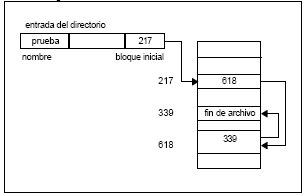
\includegraphics[width=0.5\textwidth-\fboxrule-\fboxrule]{fat.jpg}}
\end{wrapfigure}

\subsubsection{No Contiguo - Indexado}
Indexada a través de un bloque de índices que reúne a todos los apuntadores, con el objeto de ayudar el acceso director, análogo a un esquema de paginación.
\begin{itemize}
\item \textbf{Desventajas:}
\subitem + Posible desperdicio de espacio en los bloques índices.
\subitem + Tamaño del bloque índice.
\subitem + Acceso a disco necesario para recuperar la dirección del bloque para cada nivel de indexación.
\end{itemize}

\end{document}